\smallframetitle

\section{From 01/07/24 to 05/07/24}
\insertsectionframe

\begin{frame}{Introduction to the New Dataset}
    \begin{itemize}
        \item The dataset is provided by the French government and includes detailed information on radioelectrical installations with power greater than 5 watts.
        \item It is publicly accessible through the portal: \url{https://www.data.gouv.fr/fr/datasets/donnees-sur-les-installations-radioelectriques-de-plus-de-5-watts-1/}.
    \end{itemize}
    \begin{block}{Components of the Dataset}
        \begin{itemize}
            \item \textbf{SUP-ANTENNE}: Information about antennas, including dimensions, azimuths, and altitude.
            \item \textbf{SUP-BANDE}: Frequency bands used by the installations.
            \item \textbf{SUP-EMETTEUR}: Details about the emitters, including system names and service dates.
            \item \textbf{SUP-STATION}: General information about the stations, including implementation and service dates.
            \item \textbf{SUP-SUPPORT}: Support information including types and identifiers of the supports.
        \end{itemize}
    \end{block}
\end{frame}
    

\begin{frame}{Detailed Look at SUP-ANTENNE}
    \begin{block}{Fields Included}
        \begin{itemize}
            \item STA-NM-ANFR: Station identifier.
            \item AER-ID: Antenna identifier.
            \item TAE-ID: Type of antenna.
            \item AER-NB-DIMENSION: Antenna dimension.
            \item AER-FG-RAYON: Ray type.
            \item AER-NB-AZIMUT: Azimuth angle.
            \item AER-NB-ALT-BAS: Base altitude.
            \item SUP-ID: Support identifier.
        \end{itemize}
    \end{block}    

    \begin{block}{Potential Usefulness}
        \begin{itemize}
            \item Helps in understanding the physical characteristics of the antennas.
            \item Essential for modeling and simulation purposes, particularly in determining the coverage areas.
        \end{itemize}
    \end{block}
\end{frame}
    
\begin{frame}
\frametitle{Detailed Look at SUP-BANDE}
    \begin{block}{Fields Included}
        \begin{itemize}
            \item STA-NM-ANFR: Station identifier.
            \item BAN-ID: Band identifier.
            \item EMR-ID: Emitter identifier.
            \item BAN-NB-F-DEB: Start frequency.
            \item BAN-NB-F-FIN: End frequency.
            \item BAN-FG-UNITE: Frequency unit.
        \end{itemize}    
    \end{block}
    \begin{block}{Potential Usefulness}    
        \begin{itemize}
            \item Provides information on the frequency spectrum used by the installations.
            \item Crucial for interference analysis and frequency planning.
        \end{itemize}
    \end{block}    
\end{frame}
    
\begin{frame}
    \frametitle{Detailed Look at SUP-EMETTEUR}
    \begin{block}{Fields Included}
        \begin{itemize}
            \item EMR-ID: Emitter identifier.
            \item EMR-LB-SYSTEME: System label.
            \item STA-NM-ANFR: Station identifier.
            \item AER-ID: Antenna identifier.
            \item EMR-DT-SERVICE: Service date.
        \end{itemize}
    \end{block}
        
    \begin{block}{Potential Usefulness}    
        \begin{itemize}
            \item Provides operational details about the emitters.
            \item Useful for tracking the deployment and operational status of different emitters.
        \end{itemize}
    \end{block}
\end{frame}

\begin{frame}
    \frametitle{Detailed Look at SUP-STATION}
    \begin{block}{Fields Included}
        \begin{itemize}
            \item STA-NM-ANFR: Station identifier.
            \item ADM-ID: Administrator identifier.
            \item DEM-NM-COMSIS: Commune code.
            \item DTE-IMPLANTATION: Installation date.
            \item DTE-MODIF: Modification date.
            \item DTE-EN-SERVICE: Service date.
        \end{itemize}
    \end{block}
    \begin{block}{Potential Usefulness}
        \begin{itemize}
            \item Offers a comprehensive view of the station's administrative details.
            \item Important for understanding the history and modifications of each station.
        \end{itemize}
    \end{block}
\end{frame}
    
\begin{frame}{Conclusion}
            The most useful file for our research is the \textbf{SUP-ANTENNE} file.
            This file contains critical information about each antenna, including:
        \begin{block}{Useful information}
            \begin{itemize}
                \item Station identifier (STA-NM-ANFR)
                \item Antenna identifier (AER-ID)
                \item Type of antenna (TAE-ID)
                \item Antenna dimensions (AER-NB-DIMENSION)
                \item Azimuth angles (AER-NB-AZIMUT)
                \item Base altitude (AER-NB-ALT-BAS)
            \end{itemize}
        \end{block}
        \begin{block}{Methodology}
            \begin{itemize}
                \item From this data, we can extract information about the azimuth angles of antennas.
                \item This allows us to accurately calculate adjacent cells (neighbors) for each station.
            \end{itemize}
        \end{block}
\end{frame}


\begin{frame}
\frametitle{Introduction to New Methodology}
\begin{itemize}
    \item Given the valuable data from the antenne dataset, now we can take a look on a new methodology for calculating base station coverage.
    \item This methodology leverages geometric techniques and detailed information about antenna directions to improve accuracy.
    \item The approach starts with partitioning the area using Voronoi tessellation.
\end{itemize}
\end{frame}



\begin{frame}{Voronoi Tessellation}
    \begin{columns}
        \begin{column}{0.4\textwidth}
            \begin{block}{Voronoi Tessellation}
                    \begin{itemize}
                        \item The method starts by partitioning the area using Voronoi tessellation.
                        \item Each base station is a node, and its Voronoi cell contains all points closer to it than to any other base station.
                        \item The computational complexity is improved using Fortune's algorithm.
                    \end{itemize}
            \end{block}
        \end{column}
        \begin{column}{0.6\textwidth}
            \begin{figure}
                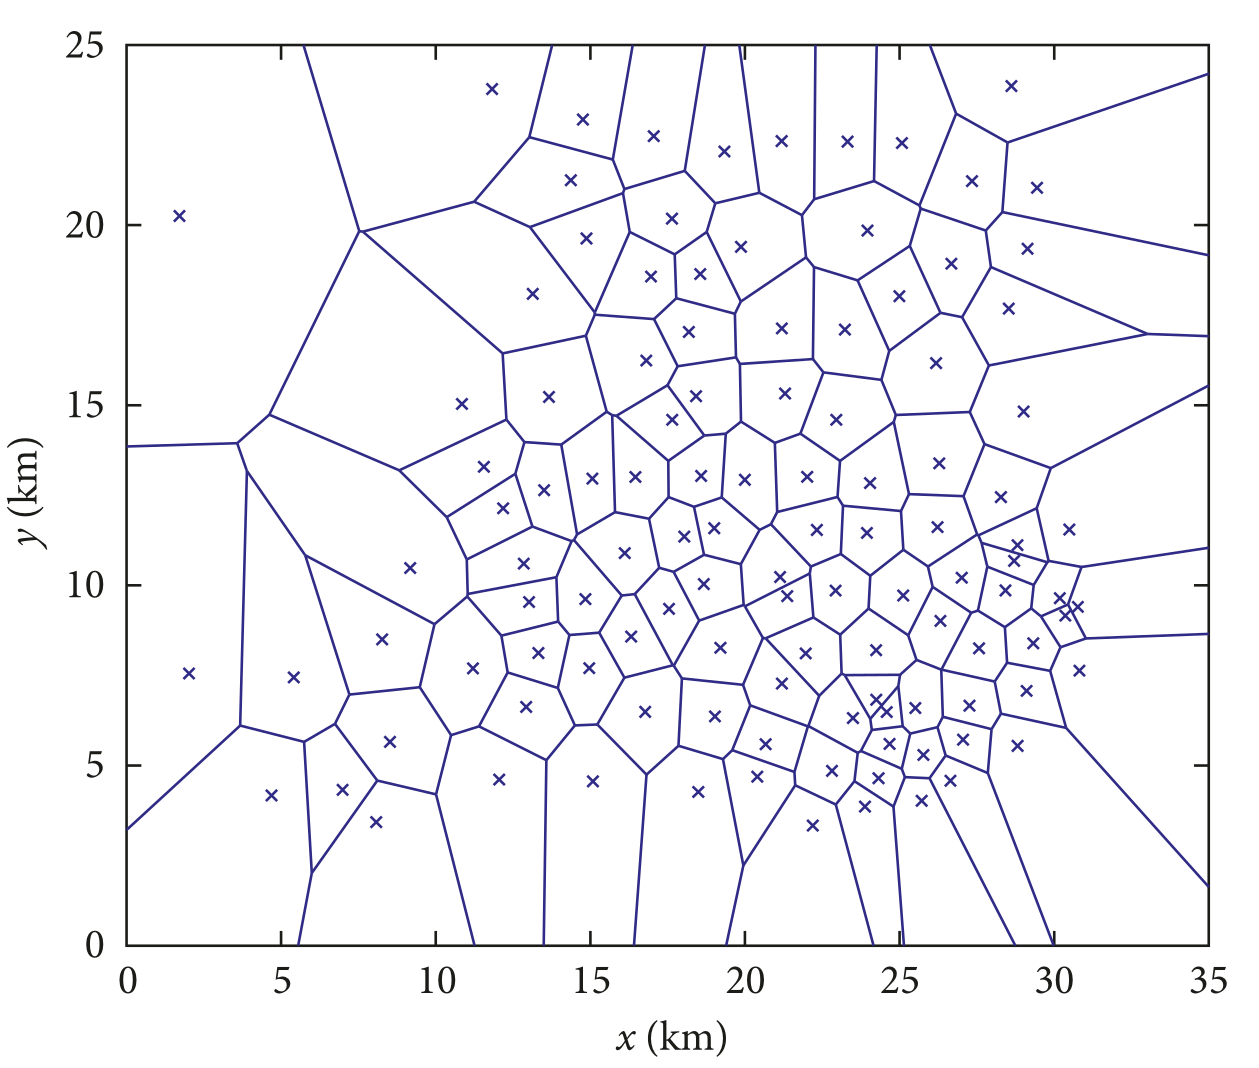
\includegraphics[width=0.7\textwidth]{images/Altair/Voronoi_appr/Voronoi_diagr.png}  % Use Figure 2 from the article
                \caption{Voronoi Diagram for Cellular Network Sites}
            \end{figure}
        \end{column}
    \end{columns}
\end{frame}




\begin{frame}{Cell Border Definition}
    \begin{columns}
        \begin{column}{0.4\textwidth}
            \begin{block}{Cell Border Definition}
                    \begin{itemize}
                        \item After generating Voronoi cells, the next step is to define cell borders based on antenna directions.
                        \item The border is defined by intersecting the Voronoi edges with the antenna beamwidth.
                        \item This process accounts for the directional nature of antennas.
                    \end{itemize}
            \end{block}
        \end{column}
        \begin{column}{0.6\textwidth}
            \begin{figure}
                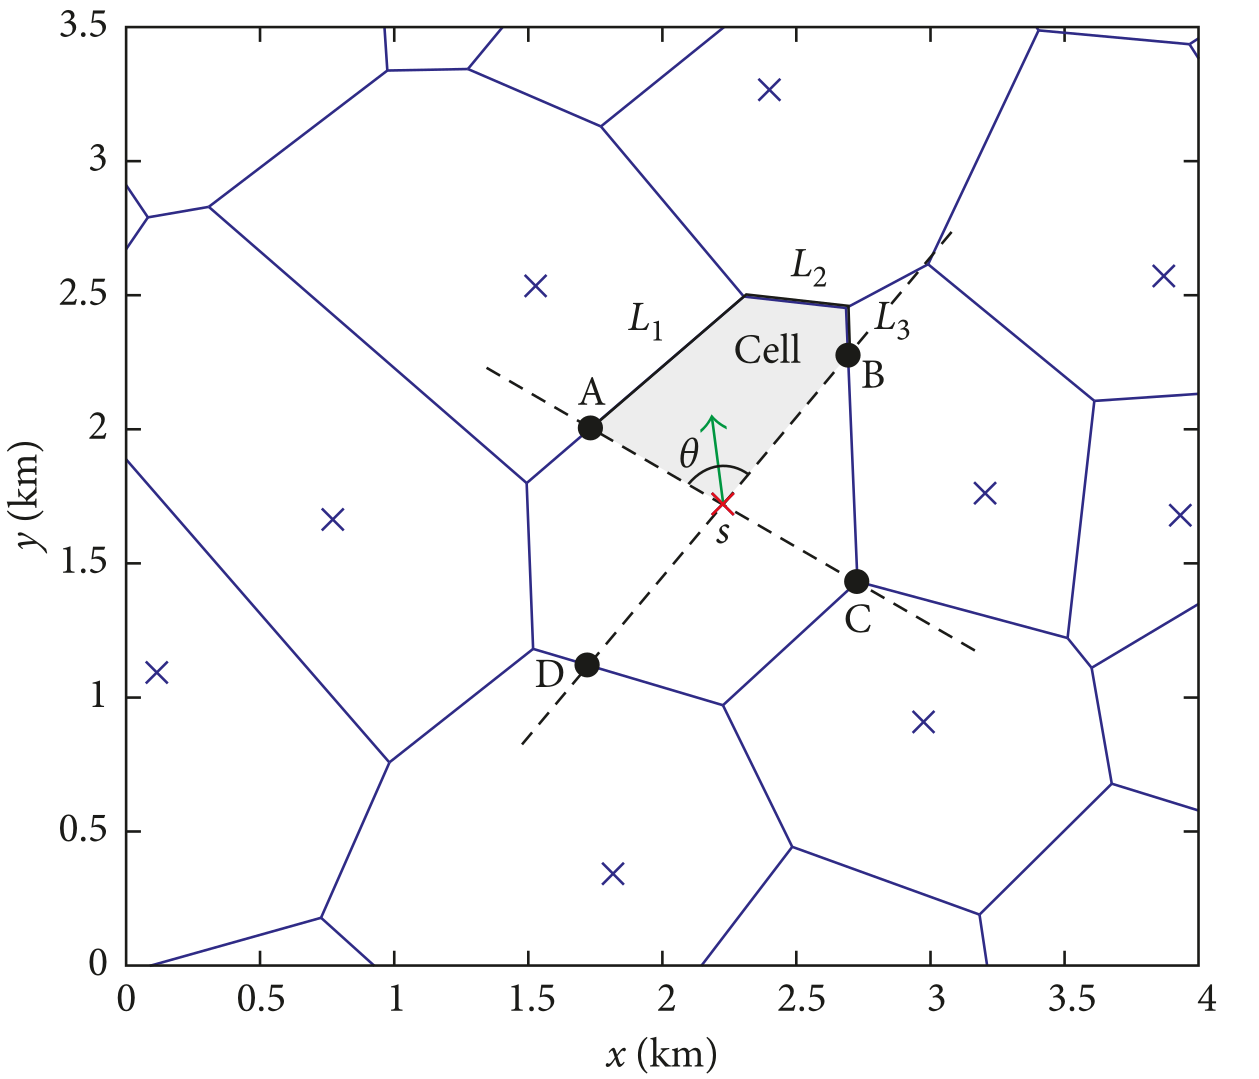
\includegraphics[width=0.7\textwidth]{images/Altair/Voronoi_appr/Cell_border.png}  % Use Figure 3 from the article
                \caption{Defining Cell Borders Using Antenna Directions}
            \end{figure}
        \end{column}
    \end{columns}
\end{frame}



\begin{frame}{Average Distance to Cell Border}
    \begin{columns}
        \begin{column}{0.55\textwidth}
            \begin{block}{Average Distance to Cell Border}
                    \begin{itemize}
                        \item The final step is to compute the average distance from the base station to the cell border.
                        \item This involves calculating the average distance to each segment of the cell border.
                        \item The formula used is:
                        \begin{equation}
                            \text{dist}(P, L) = \frac{1}{l_L} \int_0^{l_L} \sqrt{(x' - x_P')^2 + y_P'^2} \, dx'
                        \end{equation}
                        \item This ensures a weighted average distance, dominated by longer segments.
                    \end{itemize}
            \end{block}
        \end{column}
        \begin{column}{0.6\textwidth}
            \begin{figure}
                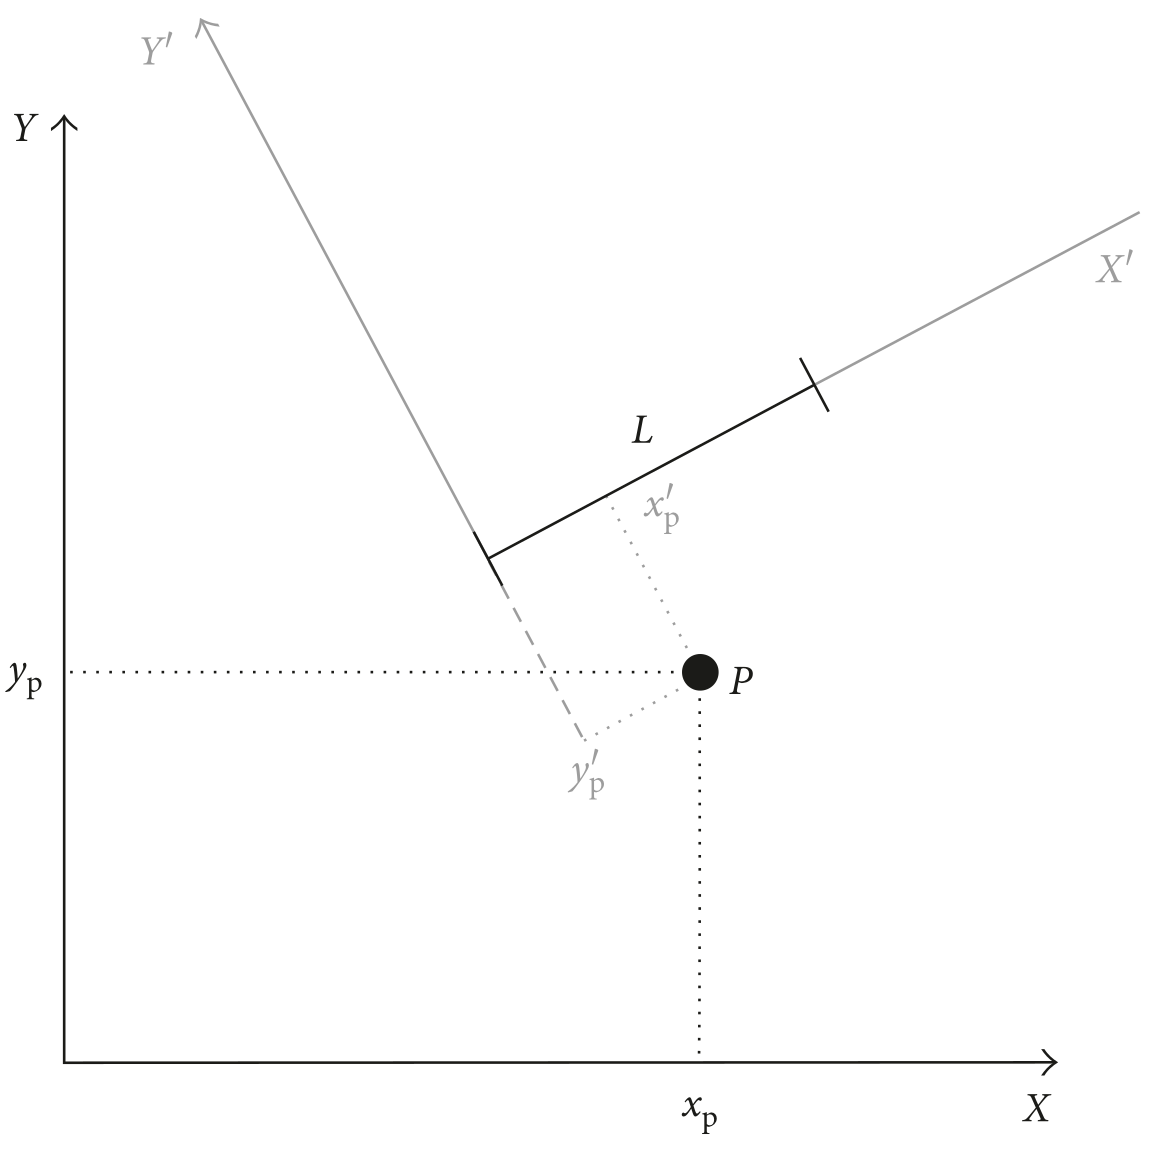
\includegraphics[width=0.5\textwidth]{images/Altair/Voronoi_appr/Point_transl.png}  % Use Figure 4 from the article
                \caption{Point Translation for Distance Calculation}
            \end{figure}
        \end{column}
    \end{columns}
\end{frame}



\begin{frame}
\frametitle{Cell Range Calculation}
\begin{itemize}
    \item The cell range (CR) for each cell is computed using:
    \begin{equation}
        \text{CR}_{\text{cell}}(c) = \frac{\sum_{i=1}^{n_{\text{seg}}(c)} \text{dist}(s, L_i) \cdot l_{L_i}}{\sum_{i=1}^{n_{\text{seg}}(c)} l_{L_i}}
    \end{equation}
    \item This method accounts for local variations and provides a more accurate estimate than site-level averages.
\end{itemize}
\begin{block}{Conclusion}
    \begin{itemize}
        \item The geometric method provides a detailed and computationally efficient way to estimate cell ranges.
        \item It addresses limitations of traditional methods by considering individual cell characteristics.
        \item This approach can be integrated into network planning and optimization processes.
    \end{itemize}
\end{block}
\end{frame}

